\documentclass[12pt,letterpaper]{article}

\usepackage{ifpdf}
\usepackage{mla}
\usepackage[utf8]{inputenc}

\begin{document}
\begin{mla}{Kyle}{Cesare}{Roush}{WR222 Section 001}{December 2, 2011}{
What Caused the Great Depression in America?}

% -- SECTION 1 --
% Introduction that hooks the reader
% Specific causal thesis with claim and reasons
The Great Depression: the longest and most severe economic depression the U.S.
experienced on this side of the Industrial Revolution.  That decade spanning
from the late 1920s to the late 1930s probably conjures up dark images of
poverty, hardship, and sadness.  But what if we could understand the causes of
the Great Depression.  And then, based on that, what if we could extrapolate
those causes to the modern day to better understand the depression we are in
now?  If we are better educated about the causes of economic disasters, perhaps
we can better defend ourselves against them in the future.  So that's the
question: what caused the Great Depression in early 20th century America?

% -- SECTION 2 --
% Body
% Significance of claim (who cares? why?)
% Evidence to support each cause or effect
% At least one image
The first thing that we must understand is that the Great Depression was a
global event with innumerable micro-causes.  A definitive cause or list of
causes would be impossible to generate.  Instead, we will analyze the events
that primarily fueled the depression.  This list is farther dwindled down by
limiting our scope to the U.S.  The depression also went against many of the
foundational ideas of classical economics.  In the introduction to John Maynard
Keynes's book, \emph{The General Theory of Employment}, it is stated that ``[The
Great Depression] led to a dramatic change in Keynes's economic thinking''
(Keynes xiv).  Keynes was a very prominent figure in economics, and essentially
established many of the priniples on which modern economics are built on.  With
neither a classical or a Keynsian model, the Great Depression was very much
uncharted territory for economists.  That said, the Great Depression was largely
caused by a combination of the stock market crashing, bank failures, and drought
conditions.

% Wall Street Crash of October, 1929 (Romer 3)
According to Christina Romer, former Chair of the Council of Economic Advisors
for the Obama administration, the first major factor that contributed to the
beginning of the Great Depression, or at least the most obvious, was the Wall
Street Crash of October, 1929.  It wouldn't have meant utter destruction, except
that the previous booming years had left investors overly optimistic.  Many
stocks were purchased on margin, which means they were bought with money taken
out as a loan.  When traders lost on these marginal bets, the problems quickly
propagated throughout the entire financial sector (``Great Depression'' 3).
Within a few years, the stock New York Stock Exchange was only a fraction of
what it was before the crash (``Great Depression 3'').

% Banking panic (Romer 3)
This initial cause set more problems in motion, one of them being panic.
Political leaders remained optimistic, but in the face of such bad news the rest
of the economy didn't hold on for much longer.  Once news of the crash made its
way to the majority of the population, everyone tried to withdraw their money
from the banking system at once.  According to Romer, banks generally only keep
a fraction of the cash on-hand, while they invest the rest in the stock market
in order to turn a profit.  These two facts led to the banks not having enough
money to fill withdrawal requests, which only perpetuated the fear and panic.
At this stage, people were losing their life savings and were surrounded by a
society falling apart, with businesses, factories, and banks all closing down
(``Great Depression'' 3).

\begin{center}
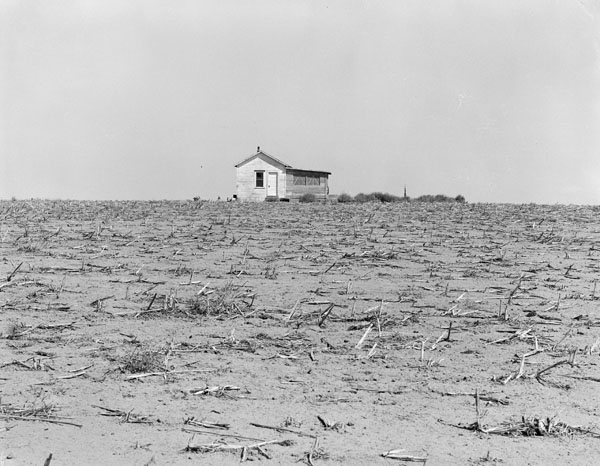
\includegraphics[width=10cm]{essay_3_dustbowl} \\
The Dust Bowl devastated America's agriculture industry (Rusinow)
\end{center}

% Prolonged by the dust bowl
Now that the depression had begun, it could only get worse.  By the mid-1930s,
severe drought conditions hit the agriculturally driven Great Planes (``About
the Dust Bowl'').  With one of America's major sectors out of play and millions
of farmers displaced, the hole of the depression only got deeper.  By mid-May
1933, \$200 million had already been allocated to help farmers refinance their
mortgages.  The spending continued with \$525 million in 1935 and \$75 million
in 1937.  Roosevelt saw ``one-third of the nation ill-housed, ill-clad,
ill-nourished... the test of our progress is not whether we add more to the
abundance of those who have much; it is whether we provide enough for those who
have too little'' (``About the Dust Bowl'').  This line was echoed in
Roosevelt's handing of the Dust Bowl, concentrating on getting people back to
work with the Works Progress Administration in 1935 and establishing such
services as the Soil Conservation Service to help farmers make it through the
tough times.

% -- SECTION 3 --
% Balance with opposition
Not everyone believes that the Great Depression was caused, in majority, by the
issues outlined above.  Some, including Milton Friedman and Anna Jacobson
Schwartz, two notable American economists, have stated that it was the Federal
Reserve's botched monetary policy that caused the Great Depression (Pongracic).
Ben Bernanke, then a Federal Reserve governor, was quoted as saying ``I would
like to say to Milton and Anna: Regarding the Great Depression, you're right.
We did it.  We're very sorry'' (Pongracic).  Obviously, this reading of the
Great Depression is backed up by very important figures, and obviously has some
merit to it.  Therefore, this area perhaps needs more research to determine
whether it truly is the cause.  In the meantime, most economists still attribute
the causes of the Great Depression to the ones outlined above.

% -- SECTION 4 --
% Relate to modern depression
Currently, we've been hearing the comparisons all over the news.  The headlines
reading ``The Great Depression: 2011'' or ``The Great Recession,'' all comparing
the modern economic situation to the Great Depression.  So, how does our modern
predicament compare with that of almost a century ago?  Well, for starters, it
isn't nearly as bad.  According to Louis Jacobson, a writer for PolitiFact and a
respected journalist, during the Great Depression, unemployment peaked at about
25\%, but unemployment today is still under 10\% (Fisk).  People are also
touting the fact that we are in the slowest recovery since the Great Depression
when, in fact, we are not.  Again, according to Jacobson, there were three
recoveries slower than today's: one under George W. Bush, one under George H.W.
Bush, and another spanning the Carter/Reagan administrations (Jacbonson).

\begin{center}
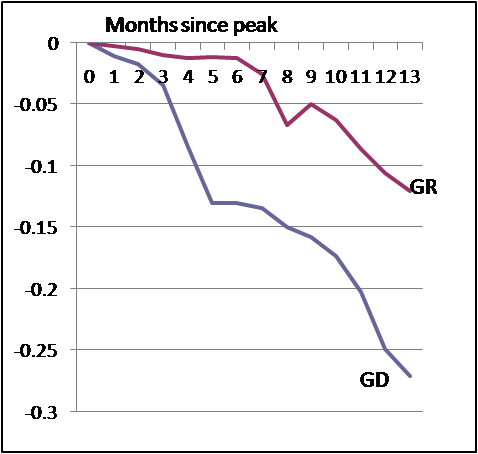
\includegraphics[width=10cm]{essay_3_gr_vs_gd} \\
The Great Depression vs. Today (Krugman)
\end{center}

The graph above, created by Paul Krugman of the New York Times, plots out the
change in industrial production as a function of the months since the peak.  It
includes two lines, one for the so called Great Recession we are in now and
another for the Great Depression.  It is by no means a stretch to say that they
are eerily similar.  However, according to Christina Romer, the depression of
today is nowhere near as bad as the Great Depression.  Even though we may hear
that we have the worst jobs numbers or worst economic indications since the
Great Depression, the GDP of the U.S. has dropped a significant 2\%, but that is
nothing compared to the 25\% drop of the Great Depression.  Even though, we can
still learn a great deal from the similarities (``Lessons from the Great
Depression for Ec.'' 1).

Another parallel we can draw is that ``today's downturn had its fundamental
cause in the decline in asset prices and the failure or near-failure of
financial institutions.  In 1929, the collapse and extreme volatility of stock''
(``Lessons from the Great Depression for Ec.'' 2) had the same effect.  Romer
points out that nearly half of all U.S. financial institutions of the 1930s
collapsed during the Great Depression; the consequences are pretty obvious.

% -- SECTION 5 --
% Conclusion
In conclusion, the Great Depression was primarily caused by a few large factors,
including but certainly not limited to, the Wall Street Crash of 1929, the
resulting bank failures and widespread panic, and the Dust Bowl in the Midwest.
Many are comparing the Great Depression with today's economic disaster, and it
appears as though such comparisons would find they had very similar causes and
effects.  Despite the similarities, make no mistake: today's ``disaster'' has
got nothin' on the Great Depression.

\begin{workscited}

% TODO: Alphabetize these

% Overview
\bibent ``About the Dust Bowl.'' \emph{Modern American Poetry}. University of
Illinois, n.d. Web. 28 Nov. 2011.

% Unemployment stats
\bibent Fisk, Donald M. ``American Labor in the 20th Century.'' \emph{Bureau of
Labor Statistics}. BLS, 30 Jan. 2003. Web. 26 Nov. 2011.

% Comparison with today
\bibent Jacobson, Louis. ``How close is today's economy to the Great
Depression?.'' \emph{PolitiFact}. N.p., 17 June 2011. Web. 26 Nov. 2011.

% Book source: Keynsian economics
\bibent Keynes, John M. \emph{The General Theory of Employment, Interest and
Money}.  New Delhi: Atlantic Publishers and Distributors, 1936. Web. 25 Nov.
2011.

\bibent Pongracic Jr., Ivan. ``The Great Depression According to Milton
Friedman.'' \emph{The Freeman Ideas on Liberty} 57.7 Sept. (2007). Web. 1 Dec.
2011.

% Scholarly source: Overview of causes, plus more
\bibent Romer, Christina D. ``Great Depression.'' University of California,
Berkeley, 20 Dec. 2003. Web. 25 Nov. 2011.

\bibent Romer, Christina D. ``Lessons from the Great Depression for Ec.''
Washington D.C. 9 Mar. 2009. Address.

\bibent Rusinow, Irving. \emph{Abandoned house, Haskell County, Kansas}. 1941.
National Archives and Records Administration. Web. 27 Nov. 2011.

\end{workscited}
\end{mla}
\end{document}
